% Version 0; preprint format; Written by SH

\documentclass[preprint]{aastex}
\usepackage{emulateapj5}
\usepackage{apjfonts}
\usepackage{amssymb, amsmath}
\usepackage{graphicx}
\usepackage{CJK}
\DeclareGraphicsExtensions{.pdf,.png,.jpg}

\input psfig.tex

%%%%%%%%%%%%: User Defined Commands %%%%%%%%%%%%

% Luis's Definitions
\def\arcsec{{\prime\prime}}
\def\arcmin{{\prime}}
\def\degree{{\circ}}
\def\h{\hskip -3 mm}
\def\aa{{A\&A}}
\def\aas{{ A\&AS}}
\def\aj{{AJ}}
\def\al{$\alpha$}
\def\bet{$\beta$}
\def\amin{$^\prime$}
\def\annrev{{ARA\&A}}
\def\apj{{ApJ}}
\def\apjs{{ApJS}}
\def\asec{$^{\prime\prime}$}
\def\deg{$^{\circ}$}
\def\ddeg{{\rlap.}$^{\circ}$}
\def\dsec{{\rlap.}$^{\prime\prime}$}
\def\cc{cm$^{-3}$}
\def\etal{{\ et al.~}}
\def\flamb{erg s$^{-1}$ cm$^{-2}$ \AA$^{-1}$}
\def\flux{erg s$^{-1}$ cm$^{-2}$}
\def\fnu{erg s$^{-1}$ cm$^{-2}$ Hz$^{-1}$}
\def\hst{{\it HST}}
\def\kms{km s$^{-1}$}
\def\lamb{$\lambda$}
\def\lax{{$\mathrel{\hbox{\rlap{\hbox{\lower4pt\hbox{$\sim$}}}\hbox{$<$}}}$}}
\def\gax{{$\mathrel{\hbox{\rlap{\hbox{\lower4pt\hbox{$\sim$}}}\hbox{$>$}}}$}}
\def\simlt{\lower.5ex\hbox{$\; \buildrel < \over \sim \;$}}
\def\simgt{\lower.5ex\hbox{$\; \buildrel > \over \sim \;$}}
\def\micron{{$\mu$m}}
\def\mnras{{MNRAS}}
\def\nat{{Nature}}
\def\pasp{{PASP}}
\def\perang{\AA$^{-1}$}
\def\peryr{yr$^{-1}$}
\def\pp{\parshape 2 0truein 6.1truein .3truein 5.5truein}
\def\reference{\noindent\pp}
\def\refindent{\par\noindent\parskip=2pt\hangindent=3pc\hangafter=1 }
\def\sb{mag~arcsec$^{-2}$}
\def\solum{$L_\odot$}
\def\solmass{$M_\odot$}


%Song Huang's definition 
\newcommand\abs[1]{\left\lvert #1 \right\rvert}
\def\galfit{{\tt GALFIT}}
\def\ser{{S\'{e}rsic\ }}
\def\mstar{$M_{\ast}$}
\def\sigstar{$\sigma_{\ast}$}
\def\m2l{$M_{\ast}/L_{\ast}$}
\def\nai{{\tt NaI}}
\def\feh{{\tt FeH}}
\def\tio{{\tt TiO}}
\def\cah{{\tt CaH}}
\def\tiO2{{\tt TiO}_{\rm 2}}

%%%%%%%%%%%%: Header and Version %%%%%%%%%%%%

\slugcomment{Draft version 0}
\shorttitle{POSSIBLE IMF GRADIENT}
\shortauthors{HUANG ET AL.}

\begin{document}

\begin{CJK*}{UTF8}{gbsn}

%%%%%%%%%%%%: Title and Affiliations %%%%%%%%%%%%

\title{Radial Gradients of Dwarf-Sensitive Spectra Features in Massive Galaxies: 
    I. Empirical Constraint from SDSS Spectra}

\author{Song Huang (黄崧)\altaffilmark{1,2,3} Luis C. Ho\altaffilmark{4,5}}
\date{}                                          

\altaffiltext{1}{Kavli Institute for the Physics and Mathematics of the
Universe, Todai Institutes for Advanced Study, the University of Tokyo (Kavli
IPMU, WPI), Kashiwa 277-8583, Japan}

\altaffiltext{2}{School of Astronomy and Space Science, Nanjing University,
Nanjing 210093, China}

\altaffiltext{3}{Key Laboratory of Modern Astronomy and Astrophysics, Nanjing
University, Nanjing 210093, China}

\altaffiltext{4}{Kavli Institute for Astronomy and Astrophysics, Peking
University, Beijing 100871, China}

\altaffiltext{5}{Department of Astronomy, School of Physics, Peking 
University, Beijing 100871, China}

%%%%%%%%%%%%: Abstract and Keywords %%%%%%%%%%%%

\begin{abstract}

* IMF-variation become an important open question regarding the stellar 
  population properties of nearby massive galaxies.  
* Although more evidence supports the relationship between the stellar 
  velocity dispersion and the central strength of several dwarf-sensitive 
  stellar absorption features, whether these features show any radial
  dependence is still a key issue to explore.  
* As most of these dwarf-sensitive features are either weak or locate in 
  NIR wavelength, it is still quite difficult to study their radial trends.
* Here, we attempt to study this by.....
* Results.   
* Diagnose of IMF is deeply integrated into the understanding of the 
  star-formation and mass-assembly history of massive galaxies. 
  
\end{abstract}

% Keywords 
\keywords{galaxies: elliptical and lenticular, cD --- galaxies: formation --- 
          galaxies: fundamental parameters --- galaxies: stellar content}

\maketitle

%%%%%%%%%%%%: Main Text %%%%%%%%%%%%

\section{Introduction}

  As an extremely important concept in astrophysics, the initial mass function 
  (IMF) can significantly influence our understanding of star and galaxy
  formation (e.g. Bastian\etal 2010; Kroupa\etal 2013).  In contrast with what 
  we used to force ourselves to believe, the ``universal'' nature of the IMF 
  was questioned in recent years.  Although the IMF is shown to be almost 
  constant across our Milky Way (e.g. Kroupa 2001) , the IMF in nearby massive
  elliptical galaxies suggested otherwise.  
  
  Since van~Dokkum \& Conroy (2010), the possible IMF variation in the center
  of nearby massive early-type galaxies (ETGs) has become an increasingly 
  exciting topic.  Motivated by the strength of the NaI $8190$\AA doublet 
  (e.g. Faber \& French 1980; Schiavon\etal 1997; referred as {\tt NaI} later)
  and the FeH Wing-Ford band around $9916$\AA (Wing \& Ford 1969; refereed as
  {\tt FeH}), the IMF was suggested to become more ``bottom-heavy'' (relative
  larger fraction of dwarf stars) at the center of massive ETGs in nearby 
  galaxy cluster.  This surprising result quickly gain more supports from 
  measurements of ``dwarf-sensitive'' absorption features in the integrated 
  spectra of nearby quiescent galaxies (e.g. van~Dokkum \& Conroy 2011; 
  Conroy \& van~Dokkum 2012, CvD12; La~Barbera\etal 2012; Spiniello\etal 2011,
  2014).  Besides the initially proposed {\tt NaI} and {\tt FeH} features,
  more promising absorption features are suggested in the near-infrared (NIR) 
  wavelength range (CvD12); Also, few more \tio and \cah related absorption 
  features are also proposed to be potentially interesting ``IMF-tracers'' in 
  the more convenient optical wavelength (La~Barbera\etal 2012; Spiniello\etal 
  2014; Chen 2014). 
  
  In stellar spectra, all these features become more prominent in dwarf stars 
  with lower effective temperature and stronger surface gravity.  Hence, in 
  the models of synthetic stellar population (SSP), the strengths of these 
  absorptions carry the information about the relative fraction of the dwarf 
  stars, and show positive correlations with the slope of IMF in the low-mass
  end.  However, none of these features is perfect.  Due to their sensitivity
  to the stellar effective temperature, many of these absorptions are also 
  very strong in low-temperature giant stars (e.g. CvD12); And, more 
  importantly, all of them show dependence on parameters like the age, total
  metallicity, $\alpha$-enhancement, or the abundance ratio of specific 
  element in the SSP models.  Many of these parameters are still poorly 
  explored.  On the bright side, developments of new stellar spectra 
  libraries (e.g. Chen\etal 2014) and SSP models (e.g. CvD12; R{\"o}ck\etal 
  2015; Vazdekis\etal 2015) will cover more parameter space better; Also, it 
  seems like that the contribution from late-type giant stars is little in 
  massive ETGs (van~Dokkum \& Conroy 2014); Initial evidence suggests that 
  the conclusions about IMF slope is not sensitive to the choice of SSP 
  models (e.g. Spiniello\etal 2015a), and is not highly degenerated with 
  the enhanced [$\alpha$/Fe] ratio in massive ETGs (McDermid\etal 2014; 
  Spiniello\etal 2015b).  

  On the other hands, efforts from both dynamical modelling (e.g., 
  Cappellari\etal 2012, 2013; Conroy et al. 2013;  Barnab{\`e}\etal 2013; 
  McDermid\etal 2014; Posacki\etal 2015) and strong-lensing constraint 
  (e.g. Treu\etal 2010; Thomas\etal 2011; Sonnenfeld\etal 2012, 2015; 
  Dutton\etal 2013; Tortora\etal 2014; Oguri\etal 2014) of the stellar 
  mass-to-light ratio (\m2l) in the inner part of massive ETGs
  also suggest that the IMF should be ``Bottom-heavier'' than the Milky-way
  like one.  The color distribution of globular clusters around nearby ETGs is 
  suggested to be consistent with ``Bottom-heavy'' IMF too (Goudfrooij \& 
  Kruijssen 2013).  Although controversial results exist from stellar 
  population (Smith\etal 2012; Worthey\etal 2011), kinematic (Clauwens\etal
  2015), strong-lensing analysis (Smith\etal 2013, 2015), and even the
  low-mass X-ray binary population (Peacock\etal 2014); And there is still 
  argument about whether results from different approaches are consistent
  with each other (Smith 2014), it seem like the extra-galactic community 
  is already quite excited about a possible new scenario where the IMF is 
  not only universal, but can even provide insights about the formation of
  these massive ETGs.  Recent works started to advance further along this 
  direction by: 
  (1). Pushing the constraint of IMF in massive galaxies into higher 
       redshift (e.g. Shetty \& Cappellari 2014; Mart{\'{\i}}n-Navarro\etal 
       2015a; Gargiulo\etal 2015); 
  (2). Searching for evidence of ``time-dependent'' IMF (e.g. Weidner\etal 
       2013; Ferreras\etal 2015); 
  (3). Investigating IMF in peculiar objects, especially the so-called 
       ``relic'' galaxies (e.g. Mart{\'{\i}}n-Navarro 2015b).  
  On the theoretical side, people has began to look into the cause of a 
  ``Bottom-heavy'' IMF (e.g. Hopkins 2013; Chabrier\etal 2014) 
  and its effect on models of galaxy formation 
  (e.g. Ferr{\'e}-Mateu\etal 2013; Fontanot 2014).  

  However, before we can draw solid conclusions in all of these 
  exciting topics, more extensive checks should be done about the 
  connection between these ``dwarf-sensitive'' absorption features
  and the IMF of the underlying stellar population, and about what is 
  the best approach to make use of them.  One particularly important
  aspect that deserve serious attention is the possible radial 
  gradient of these features. 

\section{Radial Gradient of Dwarf-Sensitive Features using 
 Aperture Effects} 
 
  Spatial distributions of stellar population properties like age, 
  metallicity, and different abundance ratios are important diagnoses 
  of massive galaxy formation.  Since the discovery of negative 
  optical color-gradient (de~Vaucouleurs 1961; Vader\etal 1988), we 
  realized that stellar population properties in massive ETGs are not 
  uniform as stars at different regions were formed at different time, 
  under changing physical condition, and assembled into the system  
  through different mergers.  Radial gradients of colors and strengths 
  of spectral features have been extensively studied 
  (e.g. S{\'a}nchez-Bl{\'a}zquez\etal 2006; La~Barbera \etal 2010; 
  Rawle\etal 2010) and were translated into gradients of age, 
  metallicity\etal.  Recent studies using new IFU instruments further 
  provide much more detailed information about the 2-dimentional 
  distribution of stellar populations (e.g. Kuntschner\etal 2010; 
  Greene\etal 2012, 2013, 2015).  In general, nearby massive ETGs 
  are known to have uniformly old stellar population age across large
  range of radii; Meanwhile, clear negative gradient of metallicity
  is another well-established conclusion.  Interestingly, it is 
  straightforward to understand these results under the increasingly 
  popular, ``two-phase'' formation scenario of massive galaxies
  (e.g. Oser\etal 2010): The inner part of massive ETGs was formed 
  through intensive star-burst at high redshift, hence the stars should
  be old, metal-rich, and $\alpha$-enhanced; while the stars in the 
  outskirts are mainly from non-dissipative mergers with less massive 
  galaxies.  As these smaller systems become the satellites of massive 
  haloes at high-redshift, the star-formation within them is expected to 
  be quenched quickly, results in old, $\alpha$-enhanced, but much 
  metal-poor stellar population.  Radial dependent mixture of these 
  two components naturally explain the gradients of stellar population. 
  
  In light of these developments, it is intriguing to ask whether the
  ``dwarf-sensitive'' features also show radial gradient like many 
  metal-sensitive features do.  If so, we should expect the slope of 
  IMF to show a radial trend as the in-situ formed stellar population 
  and the accreted one have different IMF.  However, radial gradient 
  of such features are hard to obtain.  Some of them locate in inconvenient
  wavelength range (NIR or optical-red), and are relative weak absorption
  features.  Their responses to the change of IMF are also quite small, 
  hence request spectra with high signal-to-noise ratio (at least 
  S/N$>100$) to reliably measure them.  Mart{\'{\i}}n-Navarro\etal (2015a)
  first shows a sharp negative gradient of IMF slope in massive ETG: 
  NGC~4552; And, Mart{\'{\i}}n-Navarro\etal (2015b) finds no strong 
  IMF gradient within the famous ``relic'' galaxy, NGC~1277.  Using 24 
  nearby ETGs with IFU observation from CALIFA (S{\'a}nchez\etal 2012), 
  Mart{\'{\i}}n-Navarro\etal (2015c) suggests that the IMF slope has 
  a local correlation with metallicity, implying a negative gradient 
  too.  If the IMF does has a sharp negative gradient in the central region, 
  its effect on the \m2l must be taken into account during 
  the dynamical or strong-lensing modelling; And local correlation between 
  the strength of ``IMF-tracers'' and other stellar population properties 
  make it even more important to further look into the parameter degeneracy 
  in SSP models.  In any case, it worth investigating into this using 
  statistically significant sample and high-quality spectra. 
    
  Here, we propose a novel method to detect possible radial trends of 
  these ``dwarf-sensitive'' features through the aperture effect of 
  SDSS fibre spectra.  In the redshift range between 0.05 and 0.15, 
  the massive ETGs with high central stellar velocity dispersion 
  (${\sigma}_{\ast} \sim 300$ \kms) can be treated as a uniform population 
  as there is little evolution in structure and stellar population 
  within the inner region ($\leq R_e$); only passive evolution is important 
  for the stellar population, and its effect is small during this $\sim 1.2$ 
  Gyr of time.  Meanwhile, the fixed aperture ($1.5\arcsec$ in 
  radius) of SDSS fibre naturally captures stars within different radius 
  ($\sim 1.5$ Kpc to $\sim 4.0$ Kpc), which enclose the possible region of 
  rapid change of IMF.  The relative difference of the high S/N average 
  spectra in different redshift bins can robustly tell us the existence 
  of such gradient, and its qualitative strength.  Through stacking many 
  spectra at slightly different redshift, the contamination from residual 
  of telluric OH lines can be alleviated, which is crucial to accurate 
  estimations of weak absorption features at $\lambda \ge 6000$\AA.  Here, 
  we will show the empirical results from such experiments through spectra 
  comparison and measurements of different indices.  
  
  The paper is organized as follows.  Section~2 gives brief summary of 
  sample selection and data reduction.  Section~3 shows the results from 
  comparing average spectra and absorption indices from different stellar 
  velocity dispersion and redshift bins.  And, we will discuss more 
  about the implications of possible ``IMF-gradient'' for the formation 
  history of massive galaxies in Section~4.  Future plans will be 
  discussed too.  Within this work, we assume $H_0$ = 70~km~s$^{-1}$ 
  Mpc$^{-1}$, ${\Omega}_m=0.27$, and ${\Omega}_{\Lambda}=0.73$.
  
\section{Sample Selection} 

  The parent sample is selected as $\sim 230000$ galaxies from SDSS Data 
  Release 7 (Abazajian\etal 2009) at $0.02 \le z \le 0.200$.  They are 
  required to have small error of redshift ($< 2$\%; and {\tt zWarning} 
  $=0$), clean photometry, useful \sigstar estimations ($130.0 \leq$ \sigstar
  $\le 350.0$), and small Galactic extinction ($\abs{b} \geq 10^{\degree}$; 
  $A_g \le 0.3$ mag).  Then, the sample is cross-matched with a few 
  Value-Added Catalogs to get necessary information for this work: 
  
  \begin{itemize}
      \item {\it Stellar Velocity Dispersion}, {\it Measurements of
          Emission Lines} from the {\tt OSSY} database 
          \footnote{http://gem.yonsei.ac.kr/~ksoh/wordpress/} (Oh\etal 2011): 
          it improves the origin SDSS spectral fitting using the {\tt pPXF} 
          code by Cappellari \& Emsellem (2004) to extract stellar kinematic 
          information, especially the \sigstar, and {\tt GANDALF} 
          code (Sarzi\etal 2006) to 
      \item {\it Effective Radius} from Simard\etal (2011): {\tt Gim2D} 
          fitting to large sample of nearby galaxies in SDSS using different 
          models.  We adopt the results of \ser model fitting as it describes 
          the structure of massive ETGs better than the SDSS' de~Vaucouleurs 
          model.  
      \item {\it Total Stellar Mass} form Mendel\etal (2014): \mstar 
          estimations for galaxies in Simard\etal (2011) using broad-band SED
          fitting method.  We choose to use their median total \mstar 
          from model including internal dust extinction.  A Chabrier (2003) 
          IMF is used in this work.  For massive ETGs, if the ``bottom-heavy'' IMF
          is a global property, their \mstar listed here will be systematically 
          under-estimated.  Since we only use \mstar to evaluate the properties 
          of each sub-samples, this uncertainty is not being pursued.  Roughly 
          speaking, \mstar using a Salpeter IMF is $\sim 0.25$ dex higher. 
      \item {\it Galaxy Morphology} from Huertas-Company\etal (2011) 
          that is based on machine learning algorithm.  It broadly classify 
          galaxies into a few morphology classes ({\tt E}, {\tt S0}, {\tt Sab}, 
          and {\tt Scd}).  The possibility that one galaxy is an ETG is described 
          by their {\tt pE/S0} parameter.  We choose to use {\tt pE/S0}$ > 0.7$
          as the standard to isolate ETGs.  By these definition, certain fraction 
          of disk galaxies (S0) is included, but at the high-\sigstar bins, 
          such ``contamination'' should be very moderate.  We also try more strict 
          criteria ({\tt pE}$ >  0.7$), and it leads to fewer number of galaxies 
          in each bin, but does not change the results.
  \end{itemize}
  
  After the matches, the parent sample is separated into a few redshift bins.  
  In this work, instead of narrow, constant bins of redshift, three relative 
  wide bins are used.  Problematic pixels have been masked out using the bitmasks 
  provided by SDSS.  
   
  Before we further separate them into...

  \begin{itemize}
      \item Basic sample selection from SDSS 
      \item Update velocity dispersion and other new ancillary data 
      \item Separate the sample into velocity dispersion and redshift bins 
      \item Exam the logMs-Re relations for galaxies in different redshift bins 
      \item Extra constraints from either Morphology or Emission-Line properties. 
      \item Basic properties of the samples 
      \item Especially the fraction covered by the aperture 
      \item Considering the possible under-estimation of effective radius for low-z 
    sub-sample, the actual difference in aperture fraction can be even more 
    dramatic.  
  \end{itemize}

\section{Data Reduction} 

  Each spectrum has been de-redshifted to rest-frame, and shifted from 
  SDSS' vacuum wavelength to commonly used air wavelength as most of the 
  spectral indices are defined under this system.  Galactic extinction has 
  been corrected too.  

  \begin{itemize}
      \item Spectra and the updated velocity dispersion. 
      \item Redshift- and extinction-correction 
      \item Convolve the spectra to a commonly high velocity dispersion. 
      \item Choice of normalization windows. 
      \item Errors in flux, and effect from sky emission lines.
  \end{itemize}

\subsection{Median-Combined Spectra}

Similar to other people's work, brief introduction 

\subsection{Robust-Average Spectra} 

\begin{itemize}
  \item Why using the PCA method, and the past works based on it.  
  \item Explain the code and method we used.
  \item Demonstrate the improvements through comparison 
  \item Both spectra are used for consistency check 
\end{itemize}
  
\subsection{Emission-Line Correction} 

\begin{itemize}
    \item Explain the difficulty in emission-line correction.  
    \item Explain the two options, and why we are choosing to use the fit-together
    one based on pPXF 
    \item Describe the process 
\end{itemize}

\section{Results}

\subsection{Empirical Comparison of Spectra}

\subsection{Identification of Possible IMF-sensitive Features} 

Also the velocity dispersion and redshift dependence of other spectral 
  features as a sanity check. 

\subsection{Velocity-dispersion- and Redshift-Dependence of Spectral Index}

\subsection{IMF-sensitive Index Ratio}

\section{Summary and Discussion} 

  In this work, we emphasis the importance of understanding the radial 
  dependence of ``dwarf sensitive'' absorption features in the 
  
\subsection{Effects from Passive Evolution of Stellar Population}
  
  One of the key assumption used here is that we assume that the effect of 
  passive evolution can be ignored in this $\sim 1.2$ Gyrs for old population
  when we focus on narrow spectral regions that are much more sensitive to 
  IMF than age.  Qualitatively speaking, it is a valid one for the purpose of 
  this work....
  
  Eventually this assumption will be no longer necessary when detailed IFU 
  observations of more massive galaxies are available.  However, this test 
  does bring our attention to an even more important issue.  
   
\subsection{Connection to the ``Two-Phase'' Scenario for the Formation 
of Massive Galaxies}
  
  As we have emphasised in the beginning, the diagnose of IMF within massive 
  ETGs should be integrated into the big picture of understanding the formation 
  and evolution of massive galaxies...
  
  {\tt Our plan for the next paper}
  
  {\tt Why ``Bottom-heavy'' IMF SSPs results in Younger Age}
  
\subsection{Future Directions}
  
  After looking into the spectra of massive (or high \sigstar) galaxies in SDSS, 
  it is clear that many are missing due to target selection, and they will also 
  be missed by the MaNGA survey.  Recent efforts, like Ma\etal (2014) and 
  van~den~Bosch\etal (2015), are designed to improve the situation.  Due to the 
  approximity of most galaxies in these samples, they are perfect for providing 
  a statistically complete, central reference of high \sigstar, massive galaxies 
  to be compared with results here.  They are also very suitable for detailed 
  analysis 

  Another interesting angle to extend this experiment is to look into the bulge 
  and disk of massive early-type disk galaxies.  Some bulges in nearby 
  massive S0s can also have high central \sigstar (e.g. NGC~3115's central \sigstar 
  is close to 300 \kms) and old, metal-rich stellar population, while their 
  stellar disk is believed to form in a different way and has more extended 
  star-formation history.  Whether such bulge also shows evidence of ``bottom-heavy'' 
  IMF, and whether the bulge and disk has different IMF is still open question.  
  Recently, Spiniello\etal (2015) founds the bulge and disk of a nearby disky 
  ETG both have a Milky Way-like IMF.  In van~Dokkum \& Conroy (2012) and 
  Zieleniewski\etal (2015), the inner bulge of M31 was revisited.  Although 
  enhancement in \nai feature is found, the stellar population modelling suggest
  its IMF is consistent with a Milky Way-like one.  The strong \nai is attributed 
  to enhanced [Na/Fe] though the cause of such strong enhancement is not clear. 
  It may worth looking for possible ``Bottom-heavy'' bulge or other Na-enhanced 
  bulges in SDSS and MaNGA; Also, we can extend the method used here to samples 
  of nearby S0s to learn the average trends.  Such approach should help us have 
  a more complete picture of the spatial distribution of ``dwarf-sensitive'' 
  features in massive galaxies.  

%%%%%%%%%%: Acknowledge %%%%%%%%%%
  
\acknowledgements 
   
  This work was supported by Peking University, and the Chinese 
  Academy of Science through grant No. XDB09030102 (Emergence of Cosmological 
  Structures) from the Strategic Priority Research Program and by the National 
  Natural Science Foundation of China through grant No. 11473002 (LCH), and the 
  World Premier International Research Center Initiative (WPI), MEXT, Japan 
  (SH). SH thanks Prof. Q.-S. Gu and the School of Space Science and Astronomy 
  in Nanjing University for providing long-term support.  
  
  Funding for SDSS-III has been provided by the Alfred P. Sloan Foundation, the
  Participating Institutions, the National Science Foundation, and the U.S.
  Department of Energy. The SDSS-III web site is http://www.sdss3.org.  SDSS-III
  is managed by the Astrophysical Research Consortium for the Participating
  Institutions of the SDSS-III Collaboration including the University of
  Arizona, the Brazilian Participation Group, Brookhaven National Laboratory,
  University of Cambridge, University of Florida, the French Participation
  Group, the German Participation Group, the Instituto de Astrofisica de
  Canarias, the Michigan State/Notre Dame/JINA Participation Group, Johns
  Hopkins University, Lawrence Berkeley National Laboratory, Max Planck
  Institute for Astrophysics, New Mexico State University, New York University,
  Ohio State University, Pennsylvania State University, University of
  Portsmouth, Princeton University, the Spanish Participation Group, University
  of Tokyo, University of Utah, Vanderbilt University, University of Virginia,
  University of Washington, and Yale University.

%%%%%%%%%%: Bibligraphic Section %%%%%%%%%%

\begin{thebibliography}{}

    \bibitem[Barnab{\`e} et al.(2013)]{2013MNRAS.436..253B} Barnab{\`e}, M., 
    Spiniello, C., Koopmans, L.~V.~E., et al.\ 2013, \mnras, 436, 253 

    \bibitem[Boylan-Kolchin et al.(2009)]{2009MNRAS.398.1150B} Boylan-Kolchin, 
    M., Springel, V., White, S.~D.~M., Jenkins, A., 
    \& Lemson, G.\ 2009, \mnras, 398, 1150 
  
    \bibitem[Ferr{\'e}-Mateu et al.(2013)]{2013MNRAS.431..440F} 
    Ferr{\'e}-Mateu, A., Vazdekis, A., \& de la Rosa, I.~G.\ 2013, \mnras, 431, 440 
  
    \bibitem[Gargiulo et al.(2015)]{2015A&A...573A.110G} Gargiulo, A., 
    Saracco, P., Longhetti, M., et al.\ 2015, \aap, 573, A110 
  
    \bibitem[Mart{\'{\i}}n-Navarro et al.(2015a)]{2015ApJ...798L...4M} 
    Mart{\'{\i}}n-Navarro, I., P{\'e}rez-Gonz{\'a}lez, P.~G., Trujillo, I., et 
    al.\ 2015, \apjl, 798, L4 
    
    \bibitem[Mart{\'{\i}}n-Navarro et al.(2015b)]{2015arXiv150501485M} 
    Mart{\'{\i}}n-Navarro, I., La Barbera, F., Vazdekis, A., et al.\ 2015, 
    arXiv:1505.01485 
  
    \bibitem[R{\"o}ck et al.(2015)]{2015MNRAS.449.2853R} R{\"o}ck, B., 
    Vazdekis, A., Peletier, R.~F., Knapen, J.~H., 
    \& Falc{\'o}n-Barroso, J.\ 2015, \mnras, 449, 2853 

    \bibitem[S{\'a}nchez et al.(2012)]{2012A&A...538A...8S} 
    S{\'a}nchez, S.~F., Kennicutt, R.~C., Gil de Paz, A., et al.\ 2012, \aap, 538, A8 

    \bibitem[S{\'a}nchez-Bl{\'a}zquez et al.(2006)]{2006A&A...457..823S} 
    S{\'a}nchez-Bl{\'a}zquez, P., Gorgas, J., \& Cardiel, N.\ 2006, \aap, 457, 
    823 

\end{thebibliography}{}

%%%%%%%%%%: Appendix Section %%%%%%%%%%%%

\appendix

\section{A. Summary of Stacked Spectra}

\section{B. Example of Principle Components from {\tt Robust-PCA} Method}

\section{C. Fact Sheets of Interesting Indices}

    For each index of absorption feature, we complied a concise ``fact 
    sheet'' to illustrate its dependence on param

\section{D. \nai $8190 \AA$ Features in Two Low-$z$ Samples} 

  Here, we present the atlas of colour profiles for massive elliptical 
  galaxies in our sample.  Along with the colour information for their 
  three-component models.  The format and labelling conventions are the 
  same with Figure XX and XX.  
  
%%%%%%%%%%%%: Figures Section %%%%%%%%%%%%

%Fig. 1
\clearpage
\figurenum{1}
\begin{figure}
    \centering 
    \includegraphics[width=10.5cm]{fig1.png}
    \caption{
    Relation between redshift and \sigstar (a); redshift and \mstar (b) for 
    the parent sample.  On the \sigstar figure, the boundary of each 
    subsample is highlighted by either a filled box with color (for 
    {\tt z1}, {\tt z2}, and {\tt z3}) or an empty box ({\tt z0}).  On the 
    \mstar plot, ellipses that represent the 1-$\sigma$ $z$-\mstar 
    distributions of high-\sigstar subsamples ({\tt s7} and {\tt s8}) 
    at different redshifts. 
    }
    \label{figure:1}
\end{figure}

%Fig. 2
\clearpage
\figurenum{2}
\begin{figure}
    \centering 
    \includegraphics[width=19cm]{fig2.png}
    \caption{
    Example result of average-spectrum. 
    }
    \label{figure:2}
\end{figure}

%Fig. 3
\clearpage
\figurenum{3}
\begin{figure}
    \centering 
    \includegraphics[width=19cm]{fig3.png}
    \caption{
    Example result of average-spectrum. 
    }
    \label{figure:3}
\end{figure}

%Fig. 4
\clearpage
\figurenum{4}
\begin{figure}
    \centering 
    \includegraphics[width=19cm]{fig4.png}
    \caption{
    Example result of average-spectrum. 
    }
    \label{figure:4}
\end{figure}

%Fig. 5
\clearpage
\figurenum{5}
\begin{figure}
    \centering 
    \includegraphics[width=19cm]{fig5.png}
    \caption{
    Example result of average-spectrum. 
    }
    \label{figure:5}
\end{figure}


%%% Figures for Appendix 

%Fig. A1
\clearpage
\figurenum{A1}
\begin{figure}
    \centering 
    \includegraphics[width=17cm]{figA1.png}
    \caption{
    Example result of average-spectrum. 
    }
    \label{figure:A1}
\end{figure}

%Fig. B1
\clearpage
\figurenum{B1}
\begin{figure}
    \centering 
    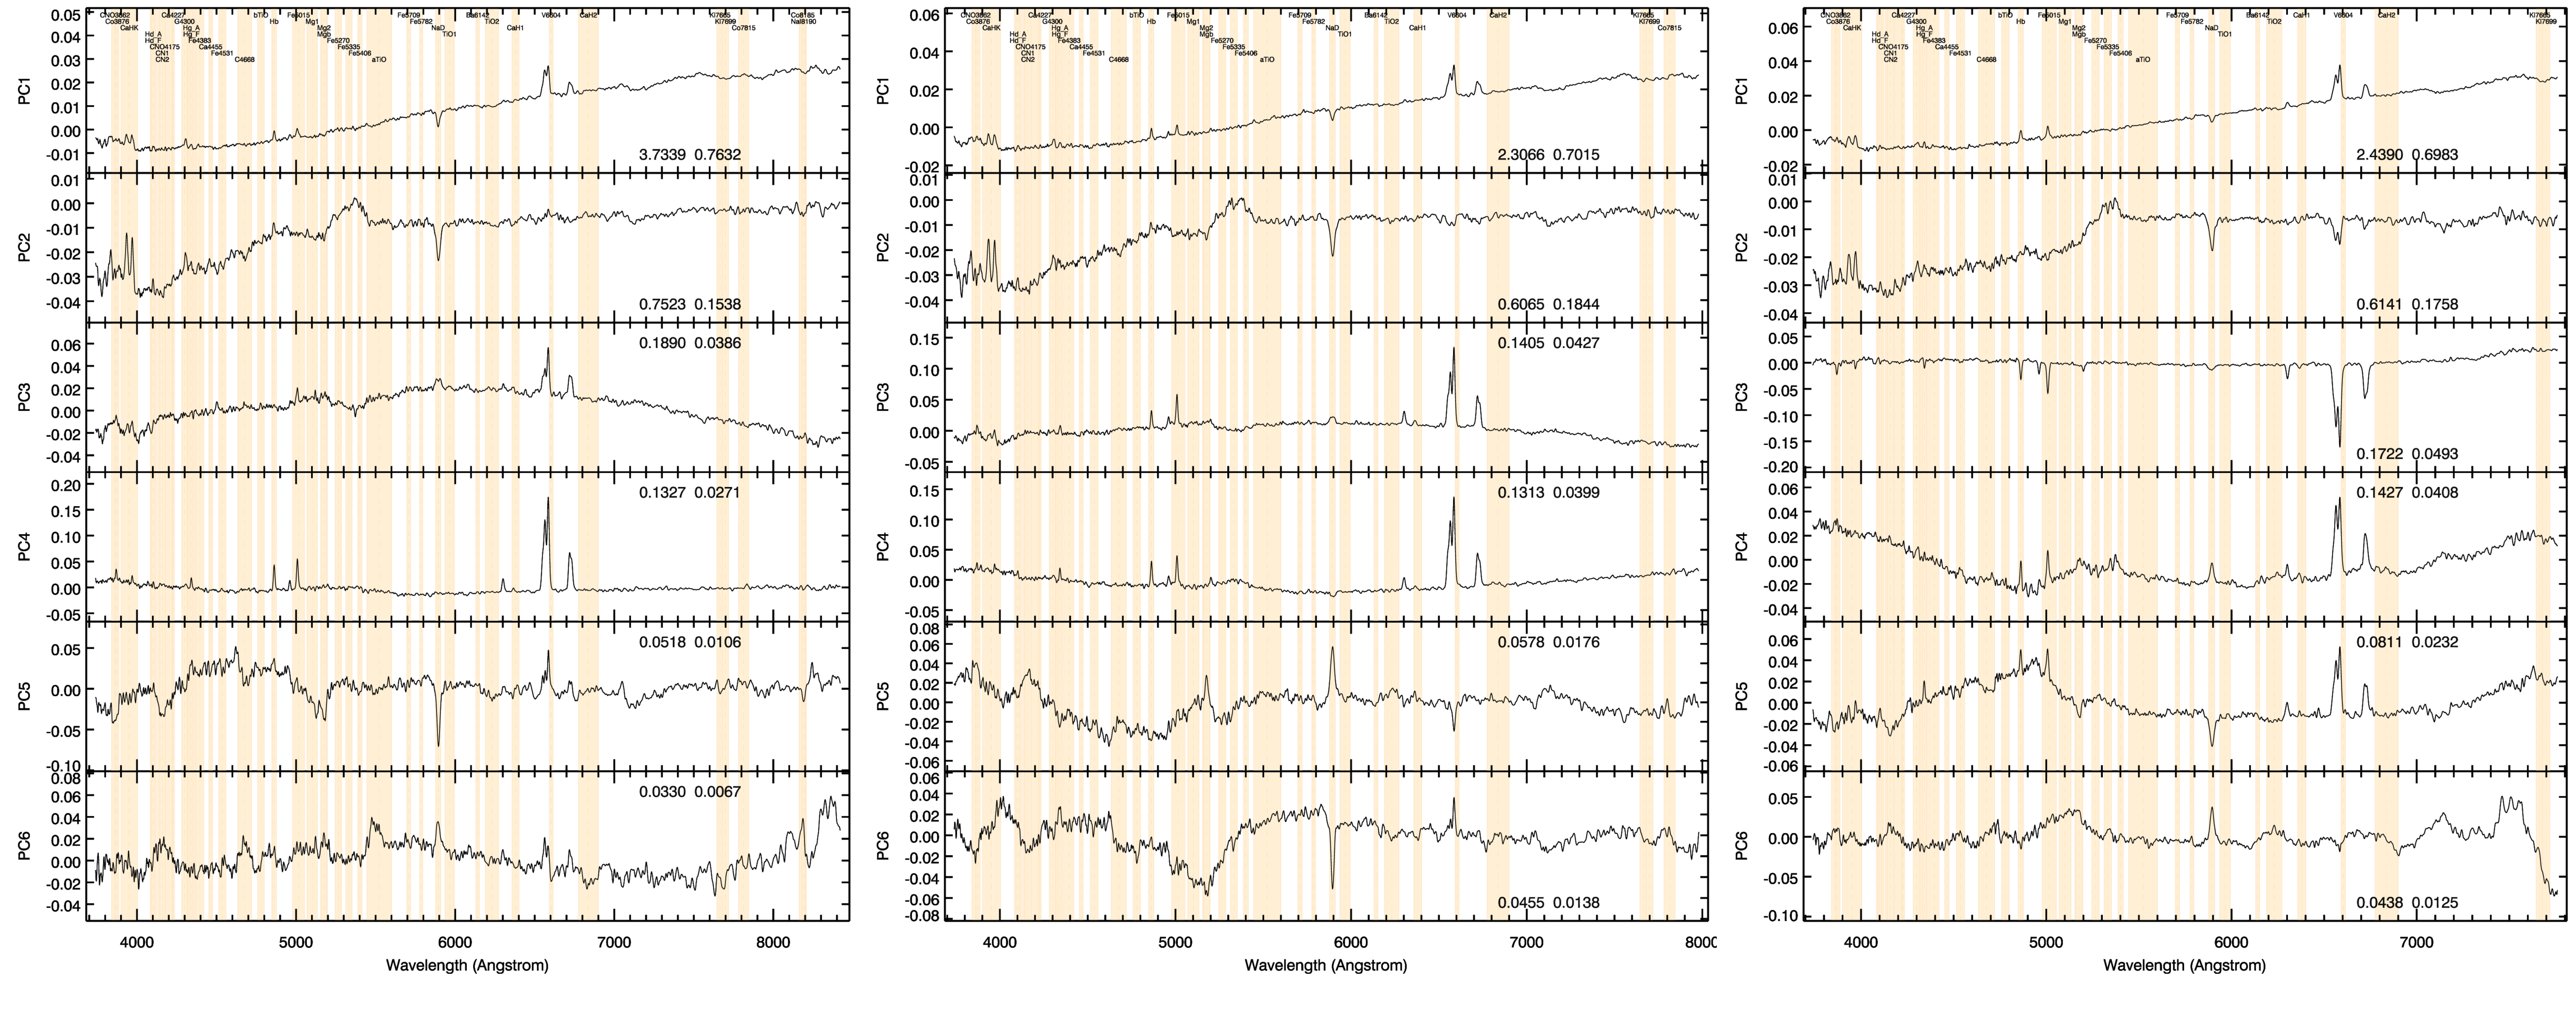
\includegraphics[width=19cm]{figB1.png}
    \caption{
    Example result of average-spectrum. 
    }
    \label{figure:B1}
\end{figure}

%Fig. C1
\clearpage
\figurenum{C1}
\begin{figure}
    \centering 
    \includegraphics[width=13cm]{figC1.png}
    \caption{
    Example result of average-spectrum. 
    }
    \label{figure:C1}
\end{figure}

%%%%%%%%%%%%: End of the File %%%%%%%%%%%%

\end{CJK*}

\clearpage 
% TABLE Summary of Samples 
% Version 0.0
%\documentstyle[apjpt4]{article}   
%\begin{document}

\def\h{\hskip -3 mm}
\def\j{\hskip -1 mm}
\def\k{\hskip -6 mm}
\def\l{\hskip -4 mm}
\def\ha{\hskip -3 mm}
\def\hb{\hskip -5 mm}
\def\hc{\hskip -3 mm}
\def\hd{\hskip -3 mm}
\def\nd{\nodata}
\def\sm{$\setminus$}
%Song Huang's definition 
\newcommand\abs[1]{\left\lvert #1 \right\rvert}
\def\galfit{{\tt GALFIT}}
\def\ser{{S\'{e}rsic\ }}
\def\mstar{$M_{\ast}$}
\def\sigstar{$\sigma_{\ast}$}
\def\m2l{$M_{\ast}/L_{\ast}$}
\def\nai{{\tt NaI}}
\def\feh{{\tt FeH}}
\def\tio{{\tt TiO}}
\def\cah{{\tt CaH}}
\def\tiO2{{\tt TiO}_{\rm 2}}

\pagestyle{empty} 
%\ptlandscape
\begin{deluxetable}{ccccccccccc}
\tabletypesize{\scriptsize}
\textheight=10.2in
\tablewidth{0pt}
%\voffset=-1.2in
%\hoffset=-0.5in
\tablecolumns{10}
%\tablewidth{9.5in}
\tablenum{1}
\tablecaption{Summary of Samples}

%%%%%%%%%%%%%%%% Table Head %%%%%%%%%%%%%%%%%%%%%

\tablehead{
    \colhead{Name} & 
    \colhead{Redshift Range} &
    \colhead{\sigstar Range} &
    \colhead{$N_{galaxy}$} &
    \multicolumn{3}{c}{$\log (M_{\ast}/M_{\odot})$} &
    \multicolumn{3}{c}{$R_e/{\rm Kpc}$} &
    \colhead{Median $S/N$}
    \nl 
    \colhead{} & 
    \colhead{} & 
    \colhead{} & 
    \colhead{} & 
    \colhead{Mean} & 
    \colhead{Stddev} & 
    \colhead{Median} &
    \colhead{Mean} & 
    \colhead{Stddev} & 
    \colhead{Median} &
    \colhead{} 
    \nl
    \colhead{    (1)} &
    \colhead{    (2)} &
    \colhead{    (3)} &
    \colhead{    (4)} &
    \colhead{    (5)} &
    \colhead{    (6)} &
    \colhead{    (7)} &
    \colhead{    (8)} &
    \colhead{    (9)} &
    \colhead{   (10)} & 
    \colhead{   (11)} 
}

\startdata

z1s1 & 0.020$-$0.075 & 140.0$-$160.0 & 1443 & 10.84 & 0.21 & 10.85 & 3.32 & 1.27 & 3.16 & 27.8 \\
z1s2 &               & 160.0$-$180.0 & 1426 & 10.93 & 0.36 & 10.95 & 3.61 & 1.30 & 3.51 & 29.3 \\ 
z1s3 &               & 180.0$-$200.0 & 1248 & 11.03 & 0.38 & 11.05 & 3.96 & 1.42 & 3.86 & 30.6 \\ 
z1s4 &               & 200.0$-$220.0 & 1143 & 11.11 & 0.40 & 11.15 & 4.27 & 1.59 & 4.17 & 31.9 \\ 
z1s5 &               & 220.0$-$240.0 &  808 & 11.21 & 0.21 & 11.22 & 4.62 & 1.58 & 4.50 & 33.4 \\ 
z1s6 &               & 240.0$-$260.0 &  542 & 11.30 & 0.22 & 11.33 & 5.03 & 1.82 & 4.87 & 34.3 \\ 
z1s7 &               & 260.0$-$290.0 &  385 & 11.40 & 0.21 & 11.41 & 5.44 & 1.82 & 5.24 & 35.6 \\ 
z1s8 &               & 290.0$-$330.0 &  146 & 11.51 & 0.18 & 11.53 & 5.99 & 1.85 & 5.81 & 36.3 \\ 

 \vspace{-1.4ex}\nl
 \cline{1-11} 
 \vspace{-1.4ex}\nl
 
z2s7 & 0.075$-$0.125 & 260.0$-$290.0 & 1337 & 11.46 & 0.21 & 11.47 & 6.76 & 2.32 & 6.52 & 25.4 \\ 
z2s8 &               & 290.0$-$330.0 &  544 & 11.57 & 0.21 & 11.59 & 7.48 & 2.48 & 7.35 & 27.5 \\ 

 \vspace{-1.4ex}\nl
 \cline{1-11} 
 \vspace{-1.4ex}\nl

z3s7 & 0.125$-$0.185 & 260.0$-$290.0 & 3207 & 11.53 & 0.18 & 11.53 & 8.16 & 2.81 & 7.77 & 17.2 \\
z3s8 &               & 290.0$-$330.0 & 1364 & 11.63 & 0.19 & 11.63 & 8.64 & 2.94 & 8.30 & 18.3 \\

 \vspace{-1.4ex}\nl
 \cline{1-11} 
 \vspace{-1.4ex}\nl

z0s7 & 0.045$-$0.090 & 260.0$-$290.0 &  663 & 11.44 & 0.20 & 11.45 & 6.62 & 1.89 & 6.40 & 32.6 \\
z0s8 &               & 290.0$-$330.0 &  290 & 11.54 & 0.19 & 11.56 & 7.25 & 2.08 & 7.10 & 33.8 \\

\enddata

%% General table comment marker
\tablecomments{Basic properties of sub-samples of nearby ETGs with SDSS 
spectra used for this work.    
Col.   (1) Name of the sample.
Col.   (2) Redshift range. 
Col.   (3) \sigstar range.
Col.   (4) Number of galaxies in the sub-sample.
Col.   (5)-(7) The mean, standard deviation, and median stellar mass of galaxies in 
           the sub-sample using estimations based on BC03 SSP models from Chen\etal (2012). 
Col.   (8)-(10) The mean, standard deviation, and median effective radius of galaxies 
           using the $r$-band single-\ser models from Simard\etal (2011).  
Col.  (11) Median $S/N$ of the spectra. 
}

%% No \tablerefs indicated
\end{deluxetable}
%\end{document}

\clearpage 
% TABLE Definition of Indices  
% Version 0.0
%\documentstyle[apjpt4]{article}   
%\begin{document}

\def\h{\hskip -3 mm}
\def\j{\hskip -1 mm}
\def\k{\hskip -6 mm}
\def\l{\hskip -4 mm}
\def\ha{\hskip -3 mm}
\def\hb{\hskip -5 mm}
\def\hc{\hskip -3 mm}
\def\hd{\hskip -3 mm}
\def\nd{\nodata}
\def\sm{$\setminus$}
%Song Huang's definition 
\newcommand\abs[1]{\left\lvert #1 \right\rvert}
\def\galfit{{\tt GALFIT}}
\def\ser{{S\'{e}rsic\ }}
\def\mstar{$M_{\ast}$}
\def\sigstar{$\sigma_{\ast}$}
\def\m2l{$M_{\ast}/L_{\ast}$}
\def\nai{{\tt NaI}}
\def\feh{{\tt FeH}}
\def\tio{{\tt TiO}}
\def\cah{{\tt CaH}}
\def\tiO2{{\tt TiO}_{\rm 2}}

\pagestyle{empty} 
%\ptlandscape
\begin{deluxetable}{ccccccc}
\tabletypesize{\scriptsize}
\textheight=10.2in
\tablewidth{0pt}
%\voffset=-1.2in
%\hoffset=-0.5in
\tablecolumns{10}
%\tablewidth{9.5in}
\tablenum{1}
\tablecaption{Wavelength Definitions of Spectral Indices}

%%%%%%%%%%%%%%%% Table Head %%%%%%%%%%%%%%%%%%%%%

\tablehead{
    \colhead{Feature} & 
    \colhead{Name} &
    \colhead{Feature Window} &
    \colhead{Blue Pseudo-continuum} &
    \colhead{Red Pseudo-continuum} &
    \colhead{Unit} &
    \colhead{Reference}
    \nl 
    \colhead{} & 
    \colhead{} & 
    \colhead{($\AA$)} & 
    \colhead{($\AA$)} & 
    \colhead{($\AA$)} & 
    \colhead{} & 
    \colhead{} 
    \nl
    \colhead{    (1)} &
    \colhead{    (2)} &
    \colhead{    (3)} &
    \colhead{    (4)} &
    \colhead{    (5)} &
    \colhead{    (6)} &
    \colhead{    (7)}
}

\startdata

TiO & {\tt LB\_TiO2}    & 6189.625-6272.125 & 6066.625-6141.625 & 6422.000-6455.000 & mag; \AA & LB13 \\
NaI  & {\tt LB\_NaI8190} & 8180.000-8200.000 & 8143.000-8153.000 & 8233.000-8244.000 & \AA & LB13 \\
TiO & {\tt SP\_bTiO}    & 4758.500-4800.000 & 4742.750-4756.500 & 4827.875-4847.875 & mag; \AA & SP13 \\
TiO & {\tt SP\_aTiO}    & 5445.000-5600.000 & 5420.000-5442.000 & 5630.000-5655.000 & mag; \AA & SP13 \\
CaH & {\tt SP\_CaH1}    & 6357.500-6401.750 & 6342.125-6356.500 & 6408.500-6429.750 & mag; \AA & SP13 \\
CaH & {\tt SP\_CaH2}    & 6775.000-6900.000 & 6510.000-6539.250 & 7017.000-7064.000 & mag; \AA & SP13 \\
TiO \& CaH & {\tt TiO\_CaH} & 6600.000-6817.000 & 6520.000-6545.000 & 7035.000-7050.000 & mag; \AA & Chen \\ 
TiO & {\tt Chen\_TiO3}   & 6600.000-6723.000 & 6520.000-6545.000 & 7035.000-7050.000 & mag; \AA & Chen \\  
CaH & {\tt Chen\_CaH}    & 6775.000-6817.000 & 6520.000-6545.000 & 7035.000 7050.000 & mag; \AA & Chen \\  

\enddata

%% General table comment marker
\tablecomments{Wavelength definitions of spectra indices used in this work.    
Col.   (1) Name of the spectra feature.
Col.   (2) Name of the index used in here. 
Col.   (3) Wavelength window forthe cetrnal feature.
Col.   (4)-(5) Blue and Red pseudo-continuum windows.
Col.   (6) Unit of the index. 
Col.   (7) Reference for original definition. LB13: La~Barbera\etal (2013); 
           SP13: Spiniello\etal (2013); Chen: Chen Ph.D. Thesis. 
}

%% No \tablerefs indicated
\end{deluxetable}
%\end{document}


\end{document}